
\section{Purpose}
To define the safe operating procedures for the Class 3B laser used for supernova calibration of the SNO+ detector. The supernova calibration source will be used as a way to predict the response of the SNO+ detector to a supernova event, acting as a "stress-test" for the detector.

\section{Description}
The laser diode in use for the SNO+ Supernova Calibration Source is a 405nm laser diode that has a peak power of approximately 240mW [1]. The laser diode is optically coupled by an optical fiber to the SNO+ laser ball that can be deployed into SNO+, externally or internally, using an Umbilical Retrival Mechanism (URM). The procedures outlined in this document should be used in conjunction with the "SNO+ Laser Ball PCA Procedures" for the deployment of the laser ball. Additional information on the supernova source components and characteristics can be found in Caitlyn Darrach's thesis[1].  
\begin{figure}[h] 
\vspace{0.5cm}
{\centering{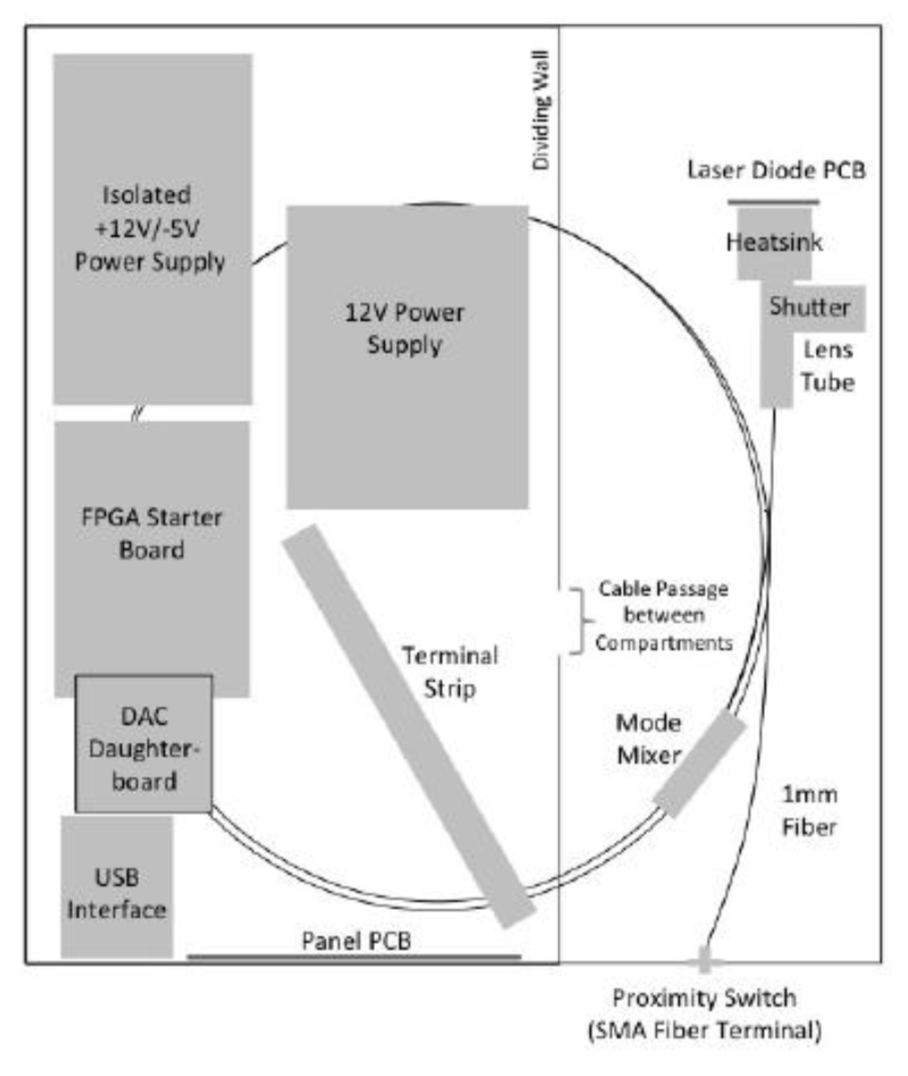
\includegraphics[height=8cm, width=8cm]{SNCDiagram.png}\par}}
\captionsetup{justification=centering}
\caption{Diagram of the components in the Supernova Source box [1]. Note that the proximity switch will automatically close the shutter if nothing is connected to it as a safety precaution.} 
\end{figure}
\section{Training}
All personnel working in the vicinity of the laser when in operation will have completed SNOLAB's \href{https://www.snolab.ca/docushare/dsweb/Get/ControlledDocument-264/SL-MCS-EHS-60-020-P-Lasers-and-UV-Irradiation-Devices-Safety-Program_Rev_01.pdf}{laser safety training} and have completed the "Laser Worker Confirmation of Training" form. An ophthalmic examination may be required. \\
Personnel should also be trained in the operation of the SNO+ calibration equipment related to the deployment of the laser ball and follow associated procedures. 

\section{Potential Hazards and Risks}
The laser in the supernova source is considered a Class 3B laser as it is a 240mW (peak power) laser. 

\underline{Eye}
\begin{itemize}
\item A Class 3B laser poses a moderate risk of eye injury if precautions aren't taken. 
\item Eye injury is possible if the retina is exposed to the beam or reflection of the beam. 
\end{itemize}

\underline{Skin}
\begin{itemize}
\item A Class 3B laser is not normally considered a skin or materials burn hazard. However, if the laser is kept motionless on skin at close range, heat can be felt. 
\end{itemize}

\section{Precautions}
\begin{itemize}
    \item Laser operators must read and understand the safe operating procedures for the laser prior to use and be trained to use lasers at SNOLAB
    \item The laser must be inspected prior to each use
    \item Ensure that there is enough time to complete all work so as to avoid rushing
    \item Avoid all exposure to the laser light
    \item Ensure that appropriate laser warning signs are displayed before the laser is operated and that all personnel in the area are aware that the laser will be in use
    \item When possible, have ambient light in the area of laser use. This keeps the pupil constricted, reducing the possibility of eye damage
    \item Keep all protective covers on the laser when in use
    \item Avoid wearing jewellery or other reflective objects during laser operation. Ensure that the area around the laser is also free from reflective surfaces
    \item Don't use the laser with a greater intensity than needed
\end{itemize}
\section{Personal Protective Equipment}
\begin{itemize}
\item Protective eye ware suitable for the wavelength of the laser must be worn at all times during the operation of the laser. 
\item Any jewellery or otherwise reflective objects should be removed 
\end{itemize}
\section{Operating Procedure}
The key for the interlock for the laser should be kept in the SNO+ Deck Clean Room (DCR) desk when not in use. \\ \\
\textbf{Pre-Operation Procedures}
\begin{enumerate}
\begin{checklist}
    \item Post laser warning signs on the door to the Deck Clean Room (DCR) including a contact name 
    \item Advise anyone already working in the area that the laser will be in use and provide appropriate laser protective goggles
    \item Check that the optical fiber is correctly connected to the source (SMA Fiber Output, see Figure 1) and that the other end is properly connected to the laser ball. The supernova calibration source has a fail-safe so that if the optical fiber is disconnected at the source box the shutter will be automatically closed. 
    \item Locate the laser interlock key and ensure that the shutter enable is in the "CLOSED" position 
\end{checklist}
\end{enumerate}
\textbf{Operation Procedures}\\
Please note that this procedure covers the operation of the Supernova Calibration laser only. This procedure should be used in conjunction with the "SNO+ Laser Ball PCA Procedures", ignoring parts that reference the N2 laser.\\ \\
\begin{figure}[h] 
\vspace{0.5cm}
{\centering{\includegraphics[height=5.5cm, width=13cm]{LabWindow.png}\par}}
\captionsetup{justification=centering}
\caption{View of the LabView user interface used to run the Supernova source and monitor its status [1].} 
\end{figure}
\begin{figure}[h] 
\vspace{0.5cm}
{\centering{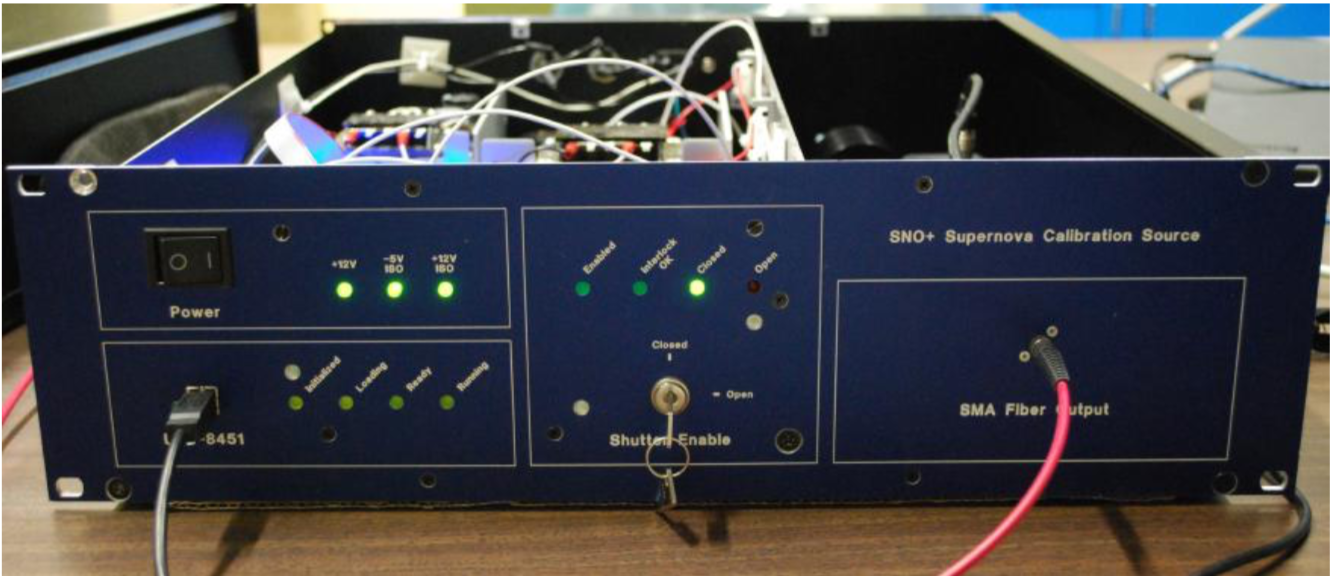
\includegraphics[height=5.5cm, width=13cm]{SNCFront.png}\par}}
\captionsetup{justification=centering}
\caption{View of the front panel of the SNO+ Supernova Calibration Source [1]. Not that the top panel is removed for this picture but would be in place during operation.} 
\end{figure}
\underline{Start-Up}
\begin{enumerate}
\begin{checklist}
    \item Log-on to the computer connected to the source (Password: s******va)
    \item Open the LabWindow program and load SNCplus
    \item Power on the supernova source
    \item Load the look up tables
    \item Set the idle DAC Value to 23,000 (activation current for the laser)
    \item Load the pulser and FIFO buffer
    \item Turn the interlock key on the source box to the "OPEN" position for the shutter
    \item Start the run by pressing "RUN" on the computer. The front panel of the laser source should display that it is "RUNNING" and that the shutter is "OPEN" (See Figure 1)
\end{checklist}
\end{enumerate}
\underline{Shut-Down}
\begin{enumerate}[resume]
\begin{checklist}
    \item Ensure that the supernova run has ended
    \item Turn the shutter interlock key to the "CLOSED" position.
    \item Power off the supernova source
    \item Save any required information
    \item Log out from the computer
\end{checklist}
\end{enumerate}
\textbf{Post-Operation Procedures}
\begin{enumerate}
\begin{checklist}
    \item Remove the key from the supernova source and return it to its designated location
    \item Remove laser warning signs and advise anyone in the area that the laser is no longer in use
\end{checklist}
\end{enumerate}
\section{Emergency Procedure}
In the event that the laser needs to be turned off quickly there is an emergency stop button located in the SNO+ control room that will stop the operation of the laser. 

\section*{Reference}
[1] Darrach, Caitlyn. {\itshape The SNO+ Supernova Calibration Source Development and Testing}. 2016.
\newline

\appendix

\section{Revision History}
\begin{center}
\begin{tabular}{|c|c|c|c|}
\hline
     \textbf{Revision} & \textbf{Date} & \textbf{Author} & \textbf{Details}  \\
     \hline
     1& & & First Draft \\
     \hline
\end{tabular}
\end{center}

\end{document}

 
